

%% 8. CUDA

\begin{frame}[fragile]{CUDA}
 
 \begin{block}{About}
  \begin{itemize}
   \item Initial release in 2007
   \item Proprietary programming model by NVIDIA
   \item C++ with extensions
   \item Proprietary compiler extracts GPU kernels
  \end{itemize}
 \end{block}

 \begin{block}{Software Ecosystem}
  \begin{itemize}
   \item Vendor-tuned libraries: cuBLAS, cuSparse, cuSolver, cuFFT, etc.
   \item Python bindings: pyCUDA
   \item Community projects: CUSP, MAGMA, VexCL, ViennaCL, etc.
  \end{itemize}
 \end{block}

\end{frame}

% Slide series: From OpenMP to CUDA. Mention shitty OpenACC?

\begin{frame}[fragile]{CUDA}
 
 \begin{block}{Programming in CUDA}
  \begin{lstlisting}
void work(double *x, double *y, double *z, int N)
{


  for (size_t i=0; i<N; ++i)
    z[i] = x[i] + y[i];
}
  \end{lstlisting}
  \begin{lstlisting}
int main(int argc, char **argv)
{
  int N = atoi(argv[1]);
  double *x = malloc(N*sizeof(double));
  ...
  
  ...
  work(x, y, z, N); // call kernel
  ...
 
 
  free(x);
}  
  \end{lstlisting}
 \end{block}
\end{frame}

%%%%%%%%%%%%%%%%%%%%5

\begin{frame}[fragile]{CUDA}
 
 \begin{block}{Programming in CUDA}
  \begin{lstlisting}
void work(double *x, double *y, double *z, int N)
{

  #pragma omp parallel for
  for (size_t i=0; i<N; ++i)
    z[i] = x[i] + y[i];
}
  \end{lstlisting}
  \begin{lstlisting}
int main(int argc, char **argv)
{
  int N = atoi(argv[1]);
  double *x = malloc(N*sizeof(double));
  ...
  
  ...
  work(x, y, z, N); // call kernel
  ...
 
 
  free(x);
}  
  \end{lstlisting}
 \end{block}
\end{frame}

%%%%%%%%%%%%%%%%%%%%5


\begin{frame}[fragile]{CUDA}
 
 \begin{block}{Programming in CUDA}
  \begin{lstlisting}
void work(double *x, double *y, double *z, int N)
{
  #pragma omp parallel
{ int thread_id = omp_get_thread_num();
  for (size_t i=thread_id; i<N; i += omp_get_num_threads())
    z[i] = x[i] + y[i];
} }
  \end{lstlisting}
  \begin{lstlisting}
int main(int argc, char **argv)
{
  int N = atoi(argv[1]);
  double *x = malloc(N*sizeof(double));
  ...
  
  ...
  work(x, y, z, N); // call kernel
  ...
 
 
  free(x);
}  
  \end{lstlisting}
 \end{block}
\end{frame}


%%%%%%%%%%%%%%%%%%%%5


\begin{frame}[fragile]{CUDA}
 
 \begin{block}{Programming in CUDA}
  \begin{lstlisting}
__global__ void work(double *x, double *y, double *z, int N)
{

  int thread_id = blockIdx.x*blockDim.x + threadIdx.x;
  for (size_t i=thread_id; i<N; i += blockDim.x * gridDim.x)
    z[i] = x[i] + y[i];
}
  \end{lstlisting}
  \begin{lstlisting}
int main(int argc, char **argv)
{
  int N = atoi(argv[1]);
  double *x = malloc(N*sizeof(double));
  cudaMalloc(&gpu_x, N*sizeof(double));
  cudaMemcpy(gpu_x, x, N*8, cudaMemcpyHostToDevice);
  ...
  work<<<128, 256>>>(x, y, z, N); // call kernel
  ...
  cudaMemcpy(gpu_x, x, N*8, cudaMemcpyDeviceToHost);
  ...
  free(x);
}  
  \end{lstlisting}
 \end{block}
\end{frame}

%%%%%%%%%%%%%%%%%%%%5

\begin{frame}[fragile]{CUDA}

 \begin{center}
  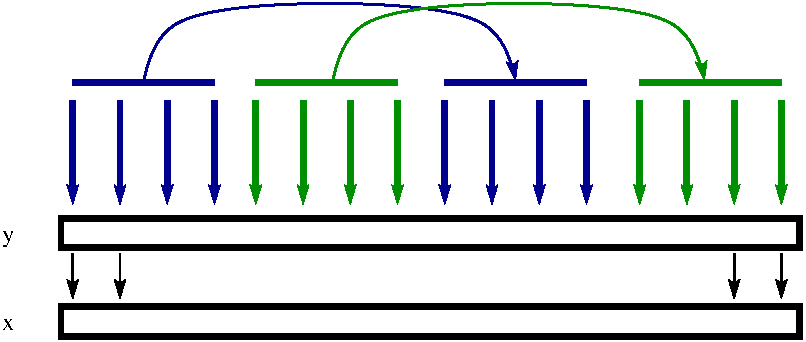
\includegraphics[width=\textwidth]{copy-kernel-gpu-full}
 \end{center}


\end{frame}

%%%%%%%%%%%%%%%%%%%%5

\begin{frame}[fragile]{CUDA}

\begin{block}{Thread Control (1D)}
 \begin{itemize}
  \item Local ID in block: \lstinline|threadIdx.x|
  \item Threads per block: \lstinline|blockDim.x|
  \item ID of block: \lstinline|blockIdx.x|
  \item No. of blocks: \lstinline|gridDim.x|
 \end{itemize}
\end{block}

\begin{block}{Recommended Default Values}
 \begin{itemize}
  \item Typical block size: 256 or 512
  \item Typical number of blocks: 256
  \item At least $10\,000$ logical threads recommended
 \end{itemize}
\end{block}

\end{frame}

%%%%%%%%%%%%%%%%%%%%5


% Revisit strided and offset memory access

\begin{frame}[fragile]{CUDA Example}

\begin{block}{Offset Memory Access}
  \begin{lstlisting}
__global__ 
void work(double *x, double *y, double *z, int N, int k)
{
  int thread_id = blockIdx.x*blockDim.x + threadIdx.x;
  for (size_t i=thread_id; i<N; i += blockDim.x * gridDim.x)
    z[i+k] = x[i+k] + y[i+k];
}  
  \end{lstlisting}
\end{block}

\vspace*{-0.5cm}
\begin{center}
 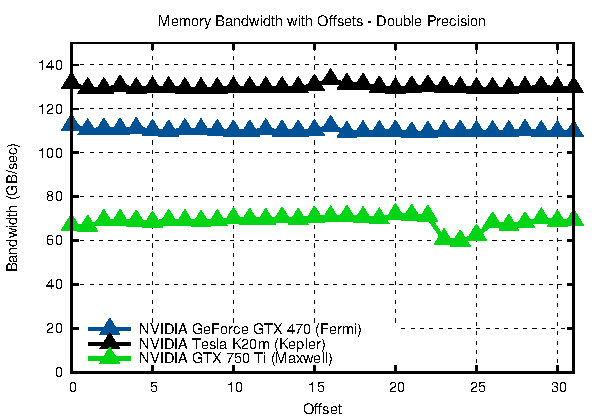
\includegraphics[width=0.6\textwidth]{figures/offset}
\end{center}

\end{frame}




\begin{frame}[fragile]{CUDA Example}

\begin{block}{Strided Memory Access}
  \begin{lstlisting}
__global__ 
void work(double *x, double *y, double *z, int N, int k)
{
  int thread_id = blockIdx.x*blockDim.x + threadIdx.x;
  for (size_t i=thread_id; i<N; i += blockDim.x * gridDim.x)
    z[i*k] = x[i*k] + y[i*k];
}  
  \end{lstlisting}
\end{block}

\vspace*{-0.5cm}
\begin{center}
 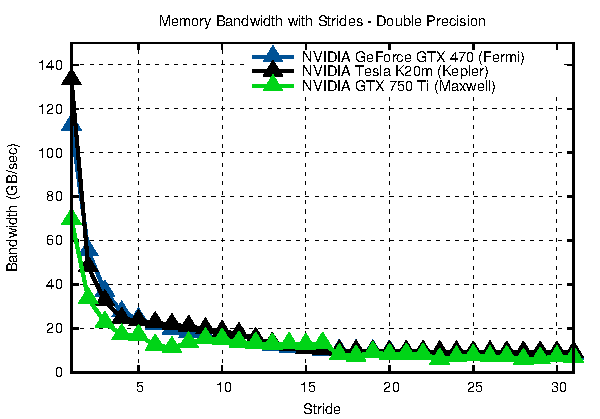
\includegraphics[width=0.6\textwidth]{figures/stride}
\end{center}

\end{frame}


%%

\begin{frame}[fragile]{CUDA Example}

\begin{block}{Strided Memory Access}
  \begin{itemize}
   \item Array of structs problematic
  \end{itemize}
  \begin{lstlisting}  
typedef struct particle
{
  double pos_x; double pos_y; double pos_z;
  double vel_x; double vel_y; double vel_z;
  double mass;
} Particle;
  
__global__ 
void increase_mass(Particle *particles, int N)
{
  int thread_id = blockIdx.x*blockDim.x + threadIdx.x;
  for (int i=thread_id; i<N; i += blockDim.x * gridDim.x)
    particles[i].mass *= 2.0;
}  
  \end{lstlisting}
\end{block}

\end{frame}

%%%

\begin{frame}[fragile]{CUDA Example}

\begin{block}{Strided Memory Access}
  \begin{itemize}
   \item Workaround: Structure of Arrays
  \end{itemize}
  \begin{lstlisting}  
typedef struct particles
{
  double *pos_x; double *pos_y; double *pos_z;
  double *vel_x; double *vel_y; double *vel_z;
  double *mass;
} Particle;
  
__global__ 
void increase_mass(Particle *particles, int N)
{
  int thread_id = blockIdx.x*blockDim.x + threadIdx.x;
  for (int i=thread_id; i<N; i += blockDim.x * gridDim.x)
    particles.mass[i] *= 2.0;
}  
  \end{lstlisting}
\end{block}

\end{frame}

